\documentclass[mathserif]{ctexbeamer}

\usepackage[orientation=landscape,size=custom,width=16,height=9,scale=0.5,debug]{beamerposter}

\usetheme{Montpellier}
\usecolortheme{spruce}

% \usepackage{beamerthemesplit} // Activate for custom appearance

% \usepackage{fontspec}

% \defaultfontfeatures{Mapping=tex-text}
\setsansfont{CMU Serif}
\setCJKsansfont{Noto Serif CJK SC}

\title{WC2020 营员交流\\
浅谈函数最值的动态维护}
\author{北京大学附属中学\quad 李白天(\emph{E.I.})}
\date{}

\newtheorem{Def}{定义}
\newtheorem{Thm}{定理}
\newtheorem{Lem}{引理}
\newtheorem{Col}{推论}

\begin{document}

\frame{\titlepage}
\section{}
\frame
{
  本人水平过于有限,以下讨论的问题极有可能并未得到最好的结果,欢迎各位之后与我交流,做出改进。
}

\section{摘要}
\frame
{
  \frametitle{摘要}

  主要对以下两个经典问题给出复杂度更好的做法:
  
  \begin{itemize}
  \item 将一个序列区间增加公差为正的等差数列,区间查询最值。本问题原本广为人知的做法为 $\Theta(\sqrt n) \Rightarrow O(\log^2 n)$。
  \item 在平面中添加一条线段,并 $\Theta(\log n)$ 查询某一 $x$ 位置上最大的 $y$ 值。操作复杂度 $\Theta(\log^2 n) \Rightarrow \Theta(\alpha(n)\log n)$,且该做法可在高次函数得到一般性的拓展。
  \end{itemize}
}

\section{引入}
\frame
{
  \frametitle{Davenport-Schinzel 序列}
  
  \begin{Def}[$(n, s)$ Davenport-Schinzel 序列]
  记一个长度为 $m$ 的序列 $\sigma_1, \sigma_2, \dots, \sigma_m$ 是一个 $(n, s)$ Davenport-Schinzel 序列(简记作 $DS(n, s)$ 序列),当且仅当 $\sigma_i$ 为 $1$ 至 $n$ 中的整数,且满足:
\begin{itemize}
\item $\sigma$ 中相邻两项值不同。
\item 对于任意 $x\neq y$,任何 $x, y$ 交替构成的序列如果是 $\sigma$ 的子序列,则长度不超过 $s+1$。
\end{itemize}
  \end{Def}
}

\frame
{
  \begin{Thm}[1]
  
  记 $\lambda_s(n)$ 为 $DS(n, s)$ 序列可能的最长长度,有\cite{ds}

$$
\lambda_s(n) = \begin{cases}
n, & s = 1 \\
2n - 1, & s = 2\\
2n\alpha(n) + O(n), & s = 3\\
\Theta(n 2^{\alpha(n)}), & s = 4\\
\Theta(n\alpha(n) 2^{\alpha(n)}), & s = 5\\
n2^{\alpha(n)^t/t! + O(\alpha(n)^{t-1})}, & s\ge 6, t = \left\lfloor \dfrac {s-2}2\right \rfloor
\end{cases}
$$

其中 $\alpha(n)$ 是反 Ackermann 函数。


  \end{Thm}
}

\subsection{DS 序列与问题的联系}

\frame
{
  \begin{Col}[1]
  对于 $n$ 个最高 $s$ 次多项式,上包络线分段长度不超过 $\lambda_s(n)$。 
  \end{Col}
  
  \begin{Col}[2]
  $n$ 个分段 $s$ 次多项式的最值的上包络线长度不超过 $\lambda_{s+2}(n)$。
  \end{Col}
  
  
在接下来的讨论中,我们将问题加以不同的特殊限制,并且在其上能够基于 $\lambda_s(n)$ 的上界设计出较为高效的算法。

\begin{enumerate}
\item 不对函数进行修改,仅作为一个集合来维护。这一限制下能够通过二进制分组的思路进行设计。
\item 询问的 $x$ 保证是单调递增的。这一限制下能够通过类似 Segment Tree Beats 的思路进行设计。
\end{enumerate}

}


\section{函数集合维护}

\frame
{
\frametitle{函数集合维护}

设有 $n$ 个函数 $f_i : \mathbb R \rightarrow \mathbb R$,对于 $x_1, x_2, \dots, x_m$ 中的每个 $x_k$,求

$$
\max_{j=1}^n f_j(x_k)
$$

当所有函数初始就被确定,我们可以分治。

}

\frame
{
每次将当前函数分成两部分进行处理,然后给得到的两组分段函数合并。复杂度即为

$$
T(n) = 2T \left(\frac n2\right) + \Theta(\lambda_s (n))
$$

根据主定理,解得 $T(n) = \Theta(\lambda_s(n) \log n)$。用于回答的时间为 $\Theta(m\log n)$。
}

\subsection{朴素实现}

\frame
{
  \frametitle{二进制分组}

  对于函数被逐一确定的情况,我们可以使用二进制分组进行处理,其实也就是对于分治的部分执行。
  
  \begin{itemize}
  \item<1->我们维护块 $L_j$ 为其中包含的 $2^j$ 个函数的上包络线所组成的分段。每当加入一个函数的时候,如果存在两个包含同样多个函数的块,就合并。

  \item<2->维护的复杂度为 $\Theta(\lambda_s(2^k)k) = \Theta(\lambda_s(n)\log n)$。

  \item<3->而对于查询,我们朴素地在每个块上二分查找到查询坐标所在的分段,时间复杂度为 $\Theta(\log^2 n)$。
  
  \item<4->考虑进一步优化。
  \end{itemize}
}

\subsection{分散层叠}

\frame
{
  \frametitle{Fractional Cascading。}
  
  我们维护辅助数组 $T_k = L_k$,对于 $0\le j< k$,将 $T_{j+1}$ 中所有 3 的倍数位置取出,与 $L_j$ 归并得到 $T_j$。同时在 $T_j$ 中记录每个元素的来源以及不同来源的前驱后继,便可以在 $\Theta(1)$ 时间内通过在 $T_j$ 中的 lowerbound 找到在 $L_j$ 和在 $T_{j+1}$ 中的 lowerbound。
  
  查询的复杂度为 $\Theta(\log n)$。
}

\frame
{
  \frametitle{维护的复杂度}
  
  由于 $|L_j| \le \lambda_s(2^j)$,且 $\lambda_s(n) = o(n^{1+\epsilon})$,可以得到 $T_j$ 的长度不超过

\begin{align*}
|T_j| & \le \sum_{t = j}^k \frac{\lambda_s(2^t)}{3^{t-j}} \\
    & = \Theta \left( \lambda_s \left( \sum_{t=0}^{k-j} \frac{2^{t+j}}{3^t} \right) \right)\\
    & = \Theta(\lambda_s(2^j))
\end{align*}


  这也是为什么不同于原始的每次除以 2 的做法,因为此处的块是等比数列。
}

\frame
{
  \frametitle{维护的复杂度}
  
  重构的复杂度为 $ \sum_{t=0}^j \Theta(\lambda_s(2^t)) = \Theta(\lambda_s(2^j))$,因此可以得到维护的总体复杂度仍然为 $\Theta(\lambda_s(n)\log n)$。
}

\subsection{应用}
\frame
{
  \frametitle{应用}

  回顾一维动态规划:  
$$
a_i = \max_{0\le j < i} a_j + w_{j,i}
$$

\begin{itemize}
\item<1->若 $a_j + w_{j, i}$ 能够改写为 $f_j(x_i)$ 的形式,且函数族 $f_i$ 交替的阶数较低,则我们可以通过上述结构进行优化转移。

\item<2->以往的这类问题中,通常需要将问题改写为一次函数的形式,或者依赖决策单调性解决。
\end{itemize}
}

\frame
{
  对于决策单调性,通常我们要求 $w$ 满足四边形不等式,从而可以得到

\begin{align*}
\forall i < j, w_{i,j+1} + w_{i+1, j} & \le w_{i,j} + w_{i+1,j+1} \\
a_i + w_{i,j+1} + a_{i+1} + w_{i+1, j} & \le a_i + w_{i,j} + a_{i+1} + w_{i+1,j+1} \\
f_i(j+1) + f_{i+1}(j) & \le f_i(j) + f_{i+1}(j + 1)\\
\Delta f_i & \le \Delta f_{i+1} \\
0 &\le \Delta (f_{i + 1} - f_i)
\end{align*}

这说明对于可以通过四边形不等式进行决策单调性优化的问题,对于 $i\le i_0$ 的函数族 $f$ 在 $j \ge i_0$ 的定义域上是 $s=1$ 阶交替的。
}

\section{决策点单调递增}

\frame
{
\frametitle{决策点单调递增}

设有 $n$ 个函数 $f_i : \mathbb R \rightarrow \mathbb R$,对于 $x_1 < x_2 < \dots < x_m$ 中的每个 $x_k$,求

$$
\max_{j=1}^n f_j(x_k)
$$

可能支持对函数的一些类型的修改?
}

\subsection{Kinetic Tournament 树}

\frame
{
\frametitle{Kinetic Tournament 树}

\begin{itemize}
\item<1->我们考虑一颗线段树,每个叶子节点表示了一个函数,线段树的每个节点存储了当前时间下子树中叶子节点的函数在当前 $x$ 下取到最大值的那个函数。

\item<2->在 $x$ 增加的过程中,我们需要不断修改某些节点的取值。

\item<3->我们维护 $x$ 变大后子树里使得某个 $\max$ 所取函数第一次发生改变的 $x$ 的值,当下一次询问超过这一 $x$ 时,我们递归下去将发生替换的部分重置。

\item<4->维护这种信息的线段树我们称为 Kinetic Tournament 树。之后我们简称为 KTT。
\end{itemize}
}

\frame
{
  \frametitle{题外话}
  
  为什么叫这个名字?
  
  \begin{itemize}
  \item<1->对于询问的 $x$ 递增的有关函数的问题,这类问题一般被称为 \textbf{Kinetic} Data Structure,询问的 $x$ 更多被称作时间,因为时间单调前进是合理的。
  \item<2->至于如何翻译这个词,“动态”一词已经被用过了……姑且从物理名词的翻译中取名“动理数据结构”,况且这类问题确实被用于物理引擎的一些应用之中。
  \end{itemize}
}

\frame
{
  \frametitle{时间复杂度}
  
  考虑每层的总复杂度 $\Theta(\lambda_s(n)\log n)$。因此直接在线段树上进行维护,本算法的复杂度为 $\Theta(\lambda_s(n)\log^2 n)$。这比直接分治要显得逊色,但是我们将要看到这一方法在更强问题上的潜力。
}

\subsection{带修改函数序列最值问题}

\frame
{
  \frametitle{带修改函数序列最值问题}
  
  考虑修改就直接类似线段树的修改方式。
  
  \begin{itemize}
  \item<1->每个叶子节点假设被修改了 $k_i$ 次,我们将其转化为这个节点下面放置 $k_i + 1$ 个节点,第一个节点是初始函数,后面接着是剩下的 $k_i$ 个函数,它们都假设是在其存在时间上的分段函数。
  
  \item<2->那么一个管辖区间为 $(l, r)$ 的节点子树里的上包络线分段数不会超过 $\lambda_{s + 2}(r - l + 1 + \sum_{i=l}^r k_i)$,因此同一层的包络线分段总和不会超过 $\lambda_{s + 2}(n + m)$。
  
  \item<3->可以做到 $\Theta(\lambda_{s + 2}(n + m)\log^2 n + q)$ 的时间内完成计算。
  
  \end{itemize}

}

\section{线性情况的扩展}

\frame
{
  \frametitle{线性情况的扩展}

  由于线性函数的性质良好,我们可以在其上研究一些扩展问题。
  
  遗憾的是,笔者暂时未能确认在更高阶情况下的类似问题维护是否有相近的复杂度。

}

\subsection{包含两类区间修改的序列最值问题}

\frame
{
  对于数列 $k_i, b_i$,我们有如下两种修改操作:

\begin{itemize}
\item 给定 $l, r, x$,对于 $l\le i\le r$,使 $b_i \leftarrow k_ix + b_i$。
\item 给定 $l, r, c, k', b'$,对于 $l\le i\le r$,使 $k_i \leftarrow ck_i + k', b_i \leftarrow cb_i + b'$。
\end{itemize}

以及进行询问一段区间上 $b_i$ 的最值。

本问题的做法改进自\cite{dzhang}。

需增加限制:\textbf{第一种修改操作中保证} $\mathbf{x > 0}$ \textbf{且第二种修改操作中保证} $\mathbf{c > 0}$。
}

\frame
{
  具体的做法思路是简单的:考虑在线段树上记录惰性标记,表示操作 2 的累计变化效果以及操作 1 的 $x$ 的累计。
  
  我们注意到操作 1 本质上就是对 KTT 上的某个节点的子树开始进行“$x$ 增大”的操作,而不是像原始的 KTT 上只从根节点进行。
  
  和 Segment Tree Beats 维护次小值有共通之处。
}

\frame
{
  \frametitle{复杂度分析}
  
  我们定义一个非叶子节点组成的集合 $\mathcal P$,对于一个非叶子节点 $v$,如果 $v$ 在当前保留的取值较大的孩子所对应的直线斜率是严格小于另一个孩子的,那么 $v\in \mathcal P$。

我们定义势函数 $\Phi = \sum_{v\in \mathcal P} d(v)$,其中 $d(v)$ 是节点 $v$ 在线段树上的深度,根节点的深度为 1。
}

\frame
{
  我们考虑 1 操作的最坏情况,即每个节点更新操作是单次进行的,那么我们定义一次更新操作的代价为 1,一次更新操作的均摊代价是 $1 + \Delta\Phi$,其中对于被修改的节点 $v$,可以得知 $v$ 必然从在 $\mathcal P$ 中变为不在,而 $v$ 的父节点 $p$ 有可能从不在 $\mathcal P$ 中变成在 $\mathcal P$ 中。故

\begin{align*}
\widehat c &= 1 + \Delta \Phi\\
&\le 1 - d(v) + d(p) \\
&= 1 - d(v) + (d(v) - 1)\\
&= 0
\end{align*}

我们这一定义使得原本无法确认进行次数的更新操作在均摊代价中不需要被考虑。

}


\frame
{
  \begin{itemize}
  
  \item<1->接下来考虑操作 1 和操作 2,它们其实本质上是类似的。
  
  \item<2->注意到当一个节点的惰性标记被修改或以其为子树的数被更新时,这一节点的父节点可能由不在 $\mathcal P$ 中变为在 $\mathcal P$ 中,这最多导致势能增加 $d(p) = \Theta(\log n)$。而一次操作会影响 $\Theta(\log n)$ 个节点,因此一次操作导致势能增加最多 $\Theta(\log^2 n)$。

  \item<3->还有一点需要注意的是由于 $\sum \widehat c_i = \sum c_i + \Phi_t - \Phi_s$,因此我们给总共的代价加上 $\Phi_s - \Phi_t = \Theta(n\log n)$,这是因为最坏情况是最初所有节点均在 $\mathcal P$ 中。

  \item<4->综上,操作过程中最多会引发 $\Theta(n\log n + m\log^2 n)$ 次更新操作,因此复杂度有上界 $O(n\log^2 n + m\log^3 n + q\log n)$。
  \end{itemize}
}

\frame
{
  \frametitle{部分特殊情况}
  
  在诸如“区间增加公差为正的等差数列”中,我们提炼出一个隐含条件:序列的 $k$ 是单调递增的。
  
  \begin{itemize}
  \item<1-> 此时我们定义势能 $\Phi$ 为“max 位于左子”的节点数。
  \item<2-> 此时操作过程最多引发 $\Theta(n + m\log n)$ 次更新操作。有复杂度上界 $O(n\log n + m\log^2 n + q\log n)$。
  \end{itemize}
}

\subsection{例题}

\subsubsection{Codeforces 573E Bear and Bowling}
\frame
{
  \frametitle{Codeforces 573E Bear and Bowling}
  
  这里只提上述数据结构相关的部分。
  
  \begin{itemize}
  \item<1->本题存在一种解法,需要按照一个顺序在一个序列 $a_n$ 中每次拿走一个数,设该数左边已经被拿走的数有 $k_i - 1$ 个,右边已经被拿走的数的总和为 $s_i$,那么每次拿的数必须是 $k_i\cdot a_i + s_i$ 中最大的。\cite{xyx}

  \item<2->如果我们使用上述的数据结构,那么只需最初令 $b_i = a_i$,每次拿走一个数后我们将 $b_i$ 加上 $-\infty$,给 $[1, i - 1]$ 这一段加上 $a_i$,给 $[i + 1, n]$ 这一段执行 $b_j \leftarrow b_j + a_j$ 即可。
  \end{itemize}
}

\subsubsection{ROI 2018 Innophone}
\frame
{
  \frametitle{ROI 2018 Innophone}
  
  \textbf{题目大意}\quad 给若干个 $x_i, y_i$,选取 $a, b$ 最大化
  
  $$ \sum_{i=1}^n [a\le x_i]a + [a > x_i][b\le y_i]b $$
  
  \textbf{做法}\quad 我们按照 $y$ 排序,扫描过程中在 KTT 上区间增加斜率,按照对应的 $y$ 值查询就可以了。
}

\subsubsection{最大连续子段和}
\frame
{
  \frametitle{最大连续子段和}
  
  对于一个数列 $a_n$,支持将区间上整体加一个正数,询问一个区间上的最大子段和。
  
  \sout{本来这也是 Ynoi2018,但是当我提出之后,lxl:那我改成可以加负数。}
}

\frame
{
  我们首先回顾没有修改操作的做法。我们在线段树的每个节点上可以维护四个值 $sum, lmax, rmax, totmax$,即可得到维护方法

\begin{align*}
sum &= ls.sum + rs.sum\\
lmax &= \max(ls.lmax, ls.sum+rs.lmax)\\
rmax &= \max(rs.rmax, rs.sum+ls.rmax)\\
totmax &= \max(ls.totmax, rs.totmax, ls.rmax + rs.lmax)
\end{align*}

  我们考虑将现在维护的这 $4$ 个信息均表示为一个一次函数。用上述的类似方法进行维护。
}

\frame
{
  \frametitle{夸张的复杂度上界。}
  
\begin{itemize}
\item<1->我们记一个包含 max 比较的变量的 rank 值 $r(v, para)$:

\item<2->对于 $r(v, lmax)$ 或 $r(v, rmax)$:对于该变量的决定式 $f(x) = \max(a(x), b(x))$,rank 值表示当前 $a, b$ 中斜率大于 $f$ 的斜率的直线的数量乘以 $d(v)^2$。
\item<3->对于 $r(v, totmax)$:对于该变量的决定式 $f(x) = \max(a(x), b(x), c(x))$,rank 值表示当前 $a, b, c$ 中斜率大于 $f$ 的斜率的直线的数量乘以 $d(v)$。

\item<4->我们直接定义势能 $\Phi = \sum_v \sum_{para} r(v, para)$。
\end{itemize}
}

\frame
{
  发生一次 $lmax$ 或 $rmax$ 的击败:
  
  $$ \Delta \Phi \le 1 -d^2 + (d-1)^2 + d-1 = 1-d \le 0 $$

  发生一次 $totmax$ 的击败:
  
  $$ \Delta \Phi \le 1 -d + d-1 = 0 $$
  
  可以得到本算法的一个复杂度上界 $O(n\log^3 n + m\log^4 n + q\log n)$,其中 $m$ 为修改次数,$q$ 为询问次数。
}

\frame
{
  \frametitle{进一步分析}
  
  \begin{itemize}
  
  
  \item<1->我们考虑每个节点的 $lmax$ 和 $rmax$ 的决策发生变化的次数。注意到 $lmax$ 的决策点只会递增,而在一个节点发生斜率切换的必要条件是决策位置从 $[l, mid]$ 切换到了 $[mid+1, r]$。每个节点最多触发一次,故 $lmax, rmax$ 的总共额外复杂度是 $\Theta(n\log n)$。

  \item<2->因此我们现在知道 KTT 维护 $lmax$ 和 $rmax$ 的总共 dfs 到的节点数是 $\Theta((n + q)\log n)$ 的。我们沿用 $totmax$ 的势能分析,复杂度是 $O((n+m)\log^3 n + q\log n)$。
  
  \item<3-> 其实之前 $\log^4 n$ 的分析可以认为是在考虑一个更 General 的操作,即加法是令 $a_i \leftarrow a_i + k_i x$,而并未考虑到 $k_i > 0$ 这一条件。
  \end{itemize}

}

\frame
{
  \frametitle{实际效率?}
  
  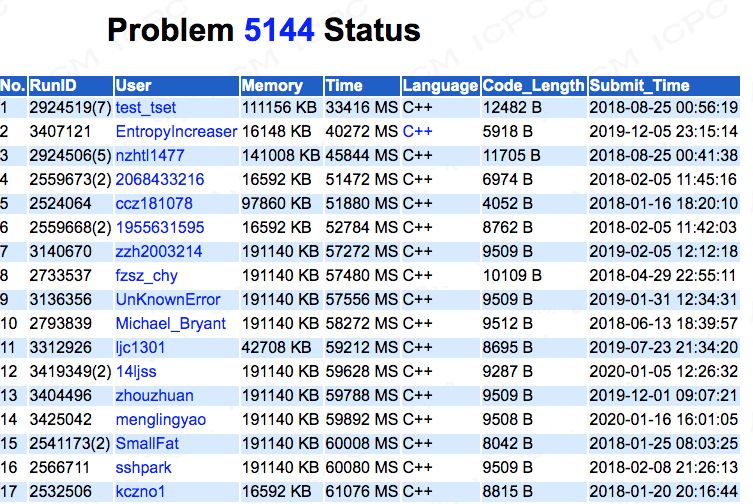
\includegraphics[width=0.4\linewidth]{image1.png}
  
  没有进行特意的卡常,但是看起来还是比较快的……
  
  可能是本身的常数因子,以及数据没有针对性等原因导致。
}

\frame
{
  \frametitle{\sout{Kinetic DDP}?}
  
  对于元素为一次函数的 $\min +$ 矩阵乘法,一般情况笔者尚未得到较好的上界。
}

\section{总结}
\frame
{
  \frametitle{总结}
  
  本文主要围绕 $DS(n,s)$ 序列本身长度的一个优秀上界,通过“减少维护的必要交点数”的方法进行设计,得到了一些复杂度比较优秀的方法用于维护函数的最值。
  
  希望本文上述的一些思路可以对 OI 中维护最值有关的问题产生更多的启发。
}

\section{参考文献}
\begin{thebibliography}{widest label}
\bibitem{ds} Micha Sharir, Pankaj K. Agarwal, \emph{Davenport-Schinzel Sequences and their Geometric Applications}, 1995
\bibitem{xyx} 徐翊轩, \emph{IOI2020中国国家集训队第一阶段作业 试题准备}, 2019
\bibitem{dzhang} Daniel Zhang, \url{https://codeforces.com/blog/entry/68534?#comment-530381}, 2019
\end{thebibliography}

\section{Q \& A}

\frame
{
  \frametitle{Q \& A}
  
  Thanks for listening.
}

\end{document}
